\documentclass{jlreq}
\usepackage[dvipdfmx]{graphicx}
\usepackage{amsmath}
\usepackage{geometry}
\usepackage{float}
\usepackage{caption}
\usepackage{hyperref}
\linespread{1.2}
\numberwithin{equation}{section}
\counterwithin{figure}{section}
\counterwithin{table}{section}

\begin{document}

\section{目的}
ゲートレベルのICを使って実際に基本ディジタル回路を作成し、動作原理について学び、理解して応用できるようにする。また、ブレッドボードの使い方を習得し、コンデンサーを用いたノイズ除去方法を学ぶ。
さらに、フリップフロップを用いたカウンタ回路やDRAM回路の動作を確認し、デジタル回路の基本的な回路の動作原理を理解する。

\section{原理}
NOT,NAND,NOR,JK-FF,D-FF について回路図と真理値表を用いて、動作や閾値などを簡潔に説明する。
NOT,NAND,NORはCMOSトランジスタを用いて記載し、JK-FFに関してはNANDを用いて記載する。

\subsection{NOTゲート}
NOTゲートは、式(2.1)のように、入力信号を反転させる基本的な論理ゲートである。入力がHIGH閾値以上のとき出力はLOWに、入力がLOW閾値未満のときは出力はHIGHになる。
\begin{equation}
  Y = \overline{A}
\end{equation}

\begin{figure}[H]
  \centering
  \begin{minipage}{0.45\textwidth}
    \centering
    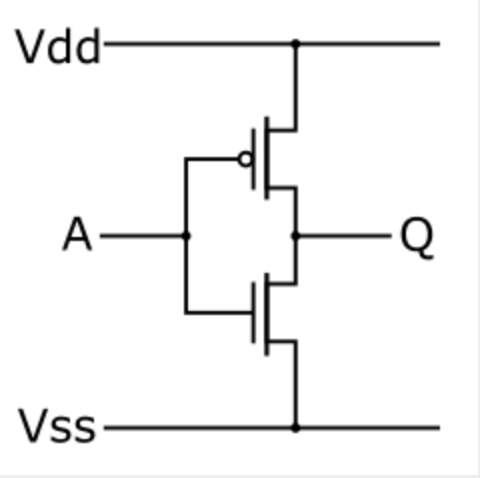
\includegraphics[width=0.8\textwidth]{assets/not.png}
    \caption{CMOSトランジスタを用いたNOTゲートの回路図}
    \label{fig:not_gate}
  \end{minipage}
  \hfill
  \begin{minipage}{0.45\textwidth}
    \centering
    \captionof{table}{NOTゲートの真理値表}
    \label{tab:not_truth_table}
    \begin{tabular}{|c|c|}
      \hline
      入力A & 出力Y \\ \hline
      0     & 1     \\ \hline
      1     & 0     \\ \hline
    \end{tabular}
  \end{minipage}
\end{figure}

\subsection{NANDゲート}
NANDゲートは、ANDゲートの出力を反転させたものである。両方の入力がHIGH閾値以上のときのみ出力がLOWとなる。

\begin{equation}
  Y = \overline{A \cdot B}
\end{equation}

\begin{figure}[H]
  \centering
  \begin{minipage}{0.45\textwidth}
    \centering
    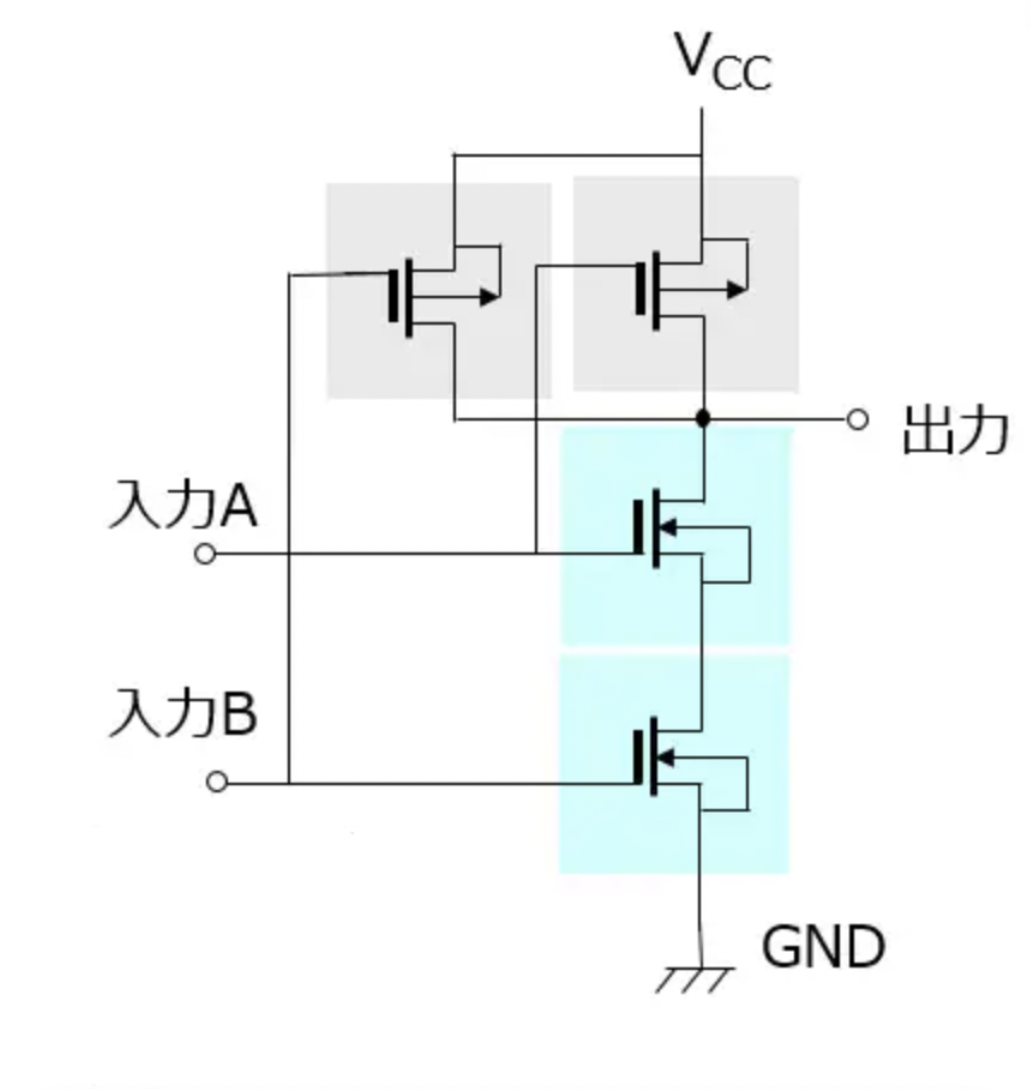
\includegraphics[width=0.8\textwidth]{assets/nand.png}
    \caption{CMOSトランジスタを用いたNANDゲートの回路図}
    \label{fig:nand_gate}
  \end{minipage}
  \hfill
  \begin{minipage}{0.45\textwidth}
    \centering
    \captionof{table}{NANDゲートの真理値表}
    \label{tab:nand_truth_table}
    \begin{tabular}{|c|c|c|}
      \hline
      入力A & 入力B & 出力Y \\ \hline
      0     & 0     & 1     \\ \hline
      0     & 1     & 1     \\ \hline
      1     & 0     & 1     \\ \hline
      1     & 1     & 0     \\ \hline
    \end{tabular}
  \end{minipage}
\end{figure}

\subsection{NORゲート}
NORゲートは、ORゲートの出力を反転させたものである。両方の入力がLOW閾値未満のときのみ出力がHIGHとなる。
\begin{equation}
  Y = \overline{A + B} 
\end{equation}

\begin{figure}[H]
  \centering
  \begin{minipage}{0.45\textwidth}
    \centering
    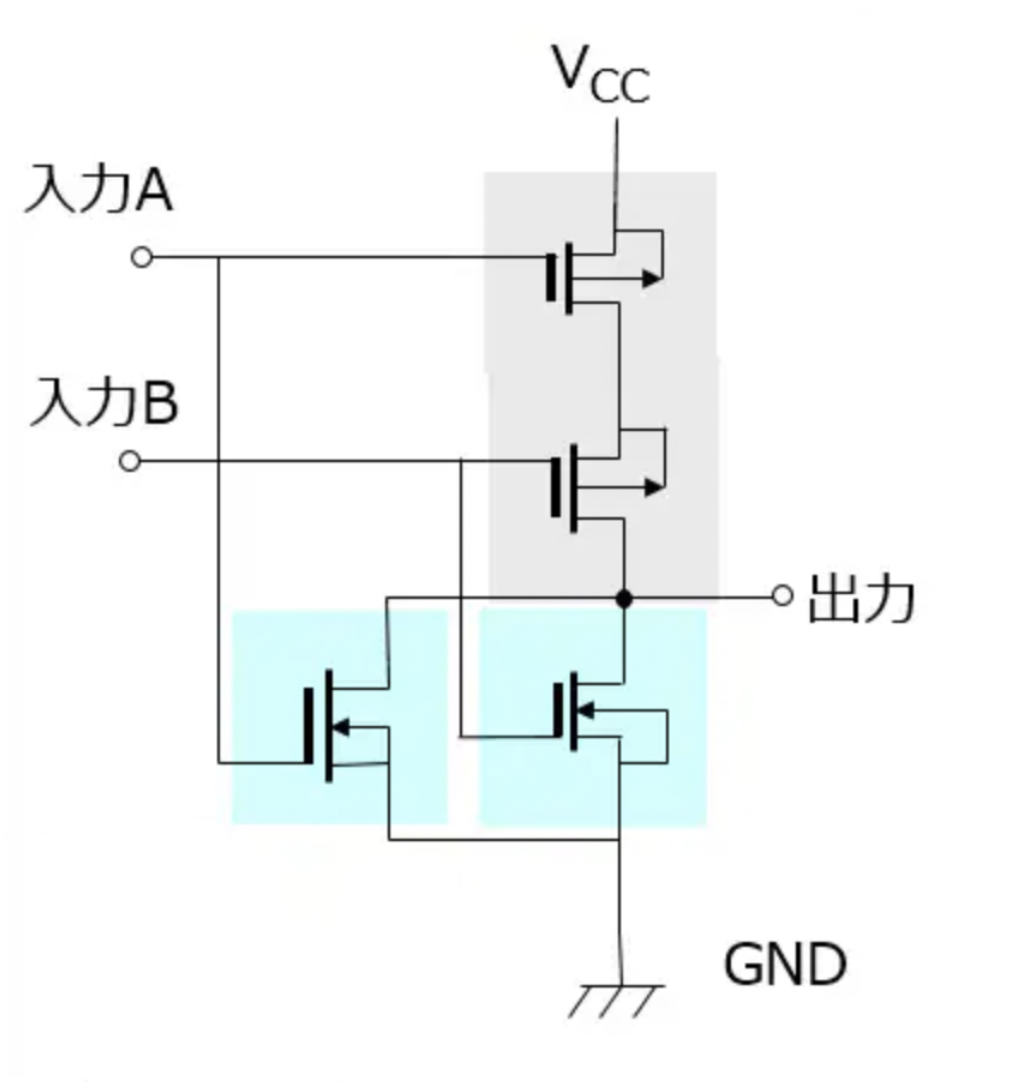
\includegraphics[width=0.8\textwidth]{assets/nor.png}
    \caption{CMOSトランジスタを用いたNORゲートの回路図}
    \label{fig:nor_gate}
  \end{minipage}
  \hfill
  \begin{minipage}{0.45\textwidth}
    \centering
    \captionof{table}{NORゲートの真理値表}
    \label{tab:nor_truth_table}
    \begin{tabular}{|c|c|c|}
      \hline
      入力A & 入力B & 出力Y \\ \hline
      0     & 0     & 1     \\ \hline
      0     & 1     & 0     \\ \hline
      1     & 0     & 0     \\ \hline
      1     & 1     & 0     \\ \hline
    \end{tabular}
  \end{minipage}
\end{figure}

\subsection{JK-FF}
JK-FFは、2つの入力信号JとKを持つフリップフロップである。クロック信号により状態が変化し、JとKの値に応じて出力Qが変化する。
\begin{equation}
  Q_{next} = J \cdot \overline{Q} + \overline{K} \cdot Q
\end{equation}

\begin{figure}[H]
  \centering
  \begin{minipage}{0.45\textwidth}
    \centering
    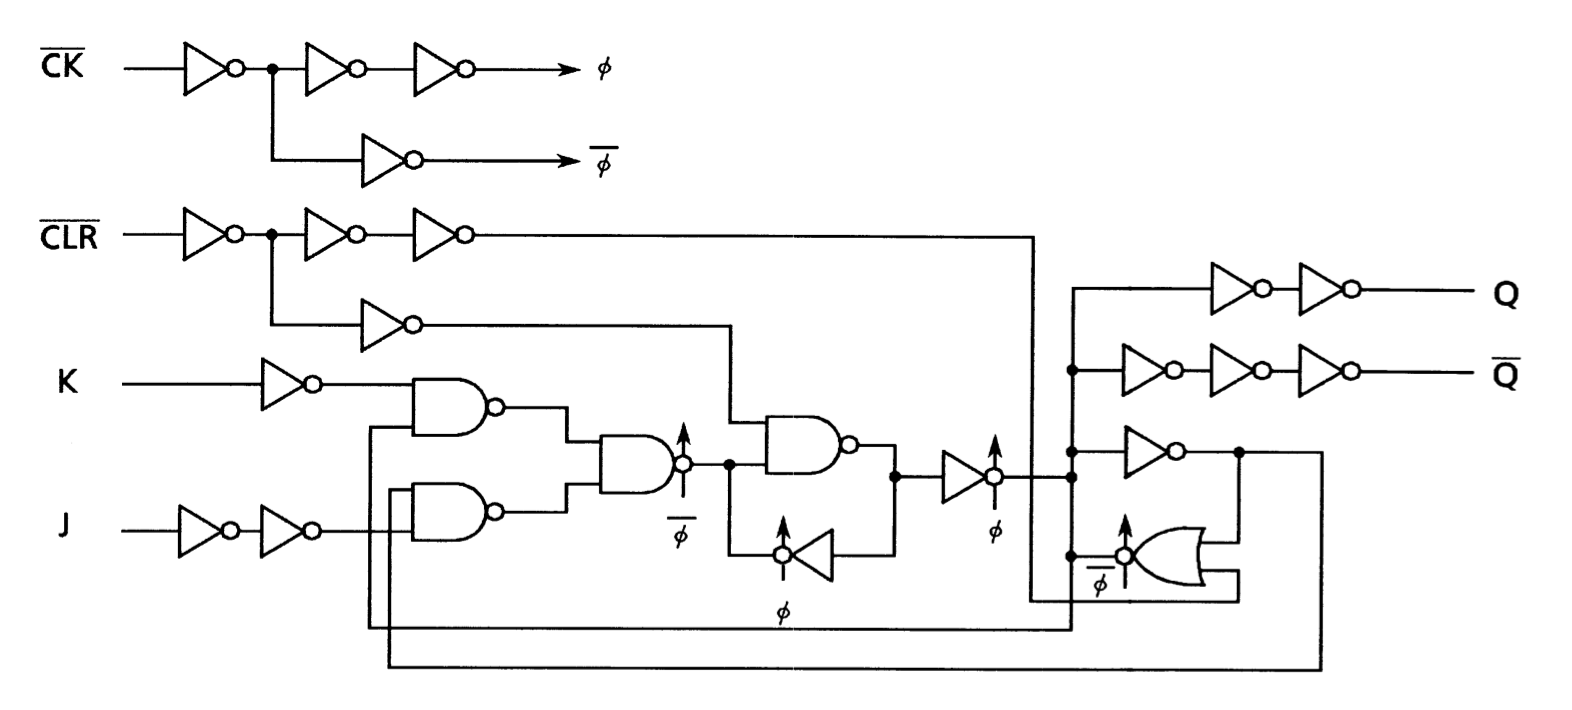
\includegraphics[width=1.2\textwidth]{assets/jk-ff.png}
    \caption{JK-FF(74HC107)の回路図}
  \end{minipage}
  \hfill
  \begin{minipage}{0.45\textwidth}
    \centering
      \captionof{table}{JK-FFの真理値表}
      \label{tab:jk_ff_truth_table}
      \begin{tabular}{|c|c|c|c|c|}
        \hline
        $\overline{\text{CLR}}$ & J & K & $\overline{\text{CK}}$ & Q, $\overline{\text{Q}}$ \\ \hline
        L & X & X & X & L, H \\ \hline
        H & L & L & $\downarrow$ & $Q_n$, $\overline{Q_n}$ \\ \hline
        H & L & H & $\downarrow$ & L, H \\ \hline
        H & H & L & $\downarrow$ & H, L \\ \hline
        H & H & H & $\downarrow$ & $\overline{Q_n}$, $Q_n$ \\ \hline
        H & X & X & $\uparrow$ & $Q_n$, $\overline{Q_n}$ \\ \hline
      \end{tabular}
  \end{minipage}
\end{figure}

クロックが立ち上がりエッジのときに、JとKの値に応じて出力Qが変化する。JとKが両方ともHIGHの場合、出力は反転する。JがHIGHでKがLOWの場合、出力はHIGHになり、JがLOWでKがHIGHの場合、出力はLOWになる。

\subsection{D-FF}
D-FFは、1つのデータ入力Dを持つフリップフロップである。クロック信号によりDの値が出力Qに転送される。JK-FFを用いてD-FFを構成できる。
\begin{equation}
  Q_{next} = D
\end{equation}
\begin{figure}[H]
  \centering
  \begin{minipage}{0.45\textwidth}
    \centering
    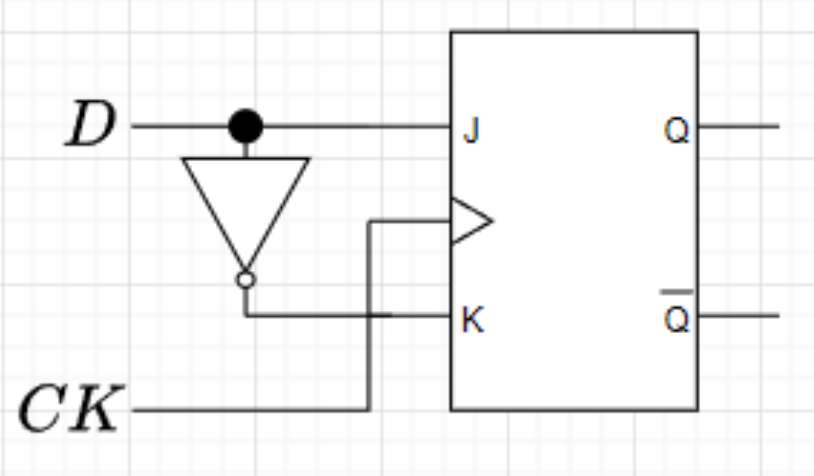
\includegraphics[width=0.8\textwidth]{assets/d-ff.png}
    \caption{D-FF(JK-FFとNOTで)の回路図}
  \end{minipage}
  \hfill
  \begin{minipage}{0.45\textwidth}
    \centering
      \captionof{table}{D-FFの真理値表}
      \label{tab:d_ff_truth_table}
      \begin{tabular}{|c|c|c|c|}
        \hline
        CK & D & Q & $\overline{Q}$ \\ \hline
        $\uparrow$ & 0 & 0 & 1 \\ \hline
        $\uparrow$ & 1 & 1 & 0 \\ \hline
      \end{tabular}
  \end{minipage}
\end{figure}
D-FFは、クロック信号の立ち上がりエッジでDの値を出力Qに転送する。クロック信号がLOWのとき、出力は前回の状態を保持する。

\subsection{シュミットトリガについて}
シュミットトリガは、入力信号の変化に対して出力信号が遅延する特性を持つ。これにより、ノイズに強く、安定した動作が可能となる。また、入力信号の上昇エッジと下降エッジで異なる閾値を持つため、ヒステリシス効果を利用しスイッチングの安定性を高めている。

\section{実験手順}
\subsection{ド・モルガンの法則の確認}


\section{実験結果}
\subsection{半加算器(HA)の結果}

\section{考察}

\section{使用機材}
\begin{itemize}
  \item オシロスコープ(型番: XXXX)
  \item 信号発生器(型番: YYYY)
  \item 電源装置(型番: ZZZZ)
\end{itemize}

\section{参考文献}
https://ushitora.net/archives/546
https://toshiba.semicon-storage.com/jp/semiconductor/knowledge/e-learning/cmos-logic-basics/chap2/chap2-2.html
https://www.marutsu.co.jp/contents/shop/marutsu/datasheet/74HC107.pdf
http://www.ctleec.sakura.ne.jp/2024/01/31/15-フリップフロップ/

\section{感想}

\end{document}